
\documentclass[xetex,professionalfont]{beamer}

\usepackage{amsmath}

\usepackage{mathtools}

\usepackage{amssymb}

\usepackage{xspace}

\usepackage{booktabs}


\usepackage{fontspec}
\setmonofont[Scale=0.7]{Droid Sans Mono} %

\usepackage[caption=false]{subfig}
\captionsetup{belowskip=0pt,aboveskip=0pt}

\usepackage{csquotes}

\usepackage{copyrightbox}

\usepackage[english]{babel}


\usepackage{tikz}

\usepackage{pgfplots}

\usetikzlibrary{backgrounds,arrows,automata}

\definecolor{xblue}{RGB}{210,224,255}
\definecolor{xyellow}{RGB}{255,255,205}
\definecolor{xred}{RGB}{255,205,205}
\definecolor{xgreen}{RGB}{205,255,205}


\hypersetup{pdftitle={DLVC Lecture 3},pdfsubject={},pdfauthor={Christopher Pramerdorfer},colorlinks,urlcolor=tuwcvl_cvl_blue,linkcolor=tuwcvl_textlight,citecolor=tuwcvl_textlight}

\makeatletter\renewcommand{\CRB@setcopyrightfont}{\tiny\color{lightgray}}

\let\oldemph\emph
\renewcommand\emph[1]{\textcolor{tuwcvl_cvl_blue}{#1}}

\usefonttheme[onlymath]{serif}

\usetheme{dlvc}


\definecolor{dred}{rgb}{0.85,0,0.1}
\definecolor{dgreen}{rgb}{0,0.85,0.1}
\definecolor{dblue}{rgb}{0,0.1,0.85}


\newcommand{\ie}{\mbox{i.e.}\xspace} %
\newcommand{\eg}{\mbox{e.g.}\xspace} %

\DeclareMathOperator*{\argmin}{arg\,min}
\DeclareMathOperator*{\argmax}{arg\,max}

\newcommand{\NN}{\mathbb{N}}
\newcommand{\ZZ}{\mathbb{Z}}
\newcommand{\QQ}{\mathbb{Q}}
\newcommand{\RR}{\mathbb{R}}

\renewcommand{\vec}[1]{\ensuremath{\mathbf{#1}}}

\newcommand{\va}{\vec{a}}
\newcommand{\vb}{\vec{b}}
\newcommand{\vc}{\vec{c}}
\newcommand{\ve}{\vec{e}}
\newcommand{\vr}{\vec{r}}
\newcommand{\vs}{\vec{s}}
\newcommand{\vt}{\vec{t}}
\newcommand{\vu}{\vec{u}}
\newcommand{\vv}{\vec{v}}
\newcommand{\vw}{\vec{w}}
\newcommand{\vx}{\vec{x}}
\newcommand{\vy}{\vec{y}}
\newcommand{\vz}{\vec{z}}
\newcommand{\vo}{\vec{o}}

\makeatletter
\let\@@magyar@captionfix\relax
\makeatother

\newcommand{\vW}{\vec{W}}
\newcommand{\bth}{\boldsymbol{\theta}}
\newcommand{\cD}{\mathcal{D}}

\DeclareMathOperator*{\sgn}{sgn}


\title{Deep Learning for Visual Computing}
\subtitle{Neural Networks \& Backpropagation}
\author{Christopher Pramerdorfer}
\institute{Computer Vision Lab, TU Wien}

\begin{document}


\begin{frame}
\maketitle
\end{frame}


\begin{frame}
  \frametitle{This Week in AI}
  \framesubtitle{Chat-GPT Plugins}
  
  \begin{center}
    \copyrightbox[b]
    {\includegraphics[width=5cm]{images/chat-plugins.jpg}}
    {\centering Image from \href{https://openai.com/}{OpenAI}}
  \end{center}
    
\end{frame}


\begin{frame}
\frametitle{Topics}

Neural networks
\begin{itemize}
    \item Motivation
    \item Computational graphs
\end{itemize}

\bigskip

Computing function gradients
\begin{itemize}
    \item Numeric and analytic gradients
    \item Derivatives in graphs
    \item Backpropagation algorithm
\end{itemize}

\end{frame}


\begin{frame}
\frametitle{Neural Networks}
\framesubtitle{Motivation}

Original idea was to roughly model neuron behavior

\bigskip

\begin{center}
    \copyrightbox[b]
    {\includegraphics[width=5.1cm]{images/neuron.png}\quad\includegraphics[width=5.1cm]{images/neuron_model.jpg}}
    {\centering Image from cs231n.github.io}
\end{center}

\end{frame}


\begin{frame}
\frametitle{Neural Networks}
\framesubtitle{Motivation}

In very simplified terms, a \emph{neuron} (nerve cell)
\begin{itemize}
    \item Has multiple input connections
    \item Weights each input signal by some factor
    \item Fires output signal if sum of inputs exceeds a threshold %
    \item Firing rate depends on sum 
\end{itemize}

\smallskip

\begin{center}
    \copyrightbox[b]
    {\includegraphics[width=6cm]{images/neuron.png}}
    {\centering Image adapted from cs231n.github.io}
\end{center}

\end{frame}


\begin{frame}
\frametitle{Neural Networks}
\framesubtitle{Motivation}

We can model this behavior as $o=a(\vw\cdot\vx+b)$
\begin{itemize}
    \item $\vx$ and $\vw$ are all inputs and weights
    \item $b$ corresponds to the threshold
    \item $a(\cdot)$ is an \emph{activation function} that models firing rate %
\end{itemize}

\smallskip

\begin{center}
    \copyrightbox[b]
    {\includegraphics[width=5.5cm]{images/neuron_model.jpg}}
    {\centering Image adapted from cs231n.github.io}
\end{center}

\end{frame}


\begin{frame}
\frametitle{Neural Networks}
\framesubtitle{Activation Functions}

We can select $a(\cdot)$ freely
\begin{itemize}
    \item \emph{Sigmoid function} $\sgn(v)$ was popular early on %
    \item \emph{Hyperbolic tangent} $\tanh(v)$ is better and sometimes used %
    \item \emph{Rectified linear unit} (\emph{ReLU}) $\max(0,v)$ most popular now %
\end{itemize}

\bigskip

Use ReLU unless you have good reason not to
\begin{itemize}
    \item We will talk more about transfer functions later
\end{itemize}

\end{frame}


\begin{frame}
\frametitle{Neural Networks}
\framesubtitle{Activation Functions}

\begin{center}
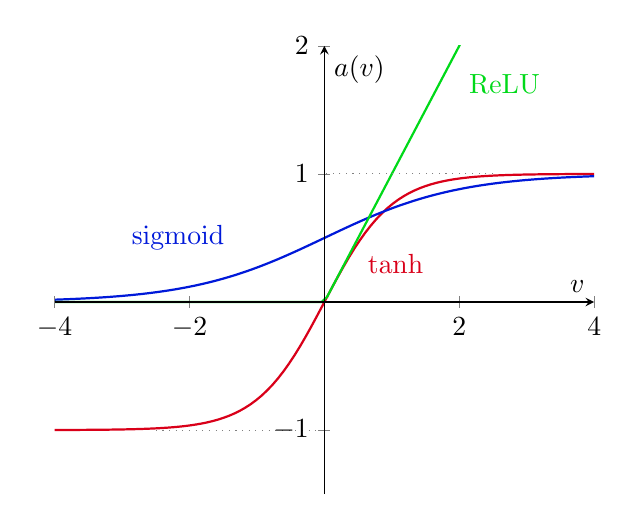
\begin{tikzpicture}
\begin{axis}[
    xmin=-4, xmax=4,
    ymin=-1.5, ymax=2,
    axis lines=center,
    axis on top=true,
    domain=-4:4,
    ylabel=$a(v)$,
    xlabel=$v$,
    samples=100
    ]

    \addplot [mark=none,draw=dred,thick] {tanh(\x)};
    \addplot [mark=none,draw=dblue,thick] {1/(1+exp(-\x))};
    \addplot [mark=none,draw=dgreen,thick] {max(0,\x)};
    \node [right, dred] at (axis cs: 0.5,0.3) {tanh};
    \node [right, dblue] at (axis cs: -3.0,0.5) {sigmoid};
    \node [right, dgreen] at (axis cs: 2.0,1.7) {ReLU};
    \draw [gray, dotted] (axis cs:-2.5,-1)-- (axis cs:0,-1);
    \draw [gray, dotted] (axis cs:+2.5,+1)-- (axis cs:0,+1);
\end{axis}
\end{tikzpicture}
\end{center}

\end{frame}


\begin{frame}
\frametitle{Neural Networks}
\framesubtitle{Activation Functions}

Use ReLU unless you have good reason not to
\begin{itemize}
    \item Performs close to optimal in wide range of tasks
    \item Helps preserve signal throughout network (more later)
    \item Results in sparse networks %
\end{itemize}

\bigskip

Several tweaks to ReLU exist (\eg Leaky ReLU, ELU)
\begin{itemize}
  \item Work (marginally) better in certain situations
\end{itemize}

  \end{frame}


\begin{frame}
\frametitle{Neural Networks}
\framesubtitle{Linear Models}

Neurons compute $o=a(\vw\cdot\vx+b)$

\bigskip

So $T$ neurons form a linear model with $T$ outputs
\begin{itemize}
    \item Simply set $a(v)=v$ such that $o_t=\vw_t\cdot\vx+b_t$
    \item Result is identical to definition in previous lecture
\end{itemize}

\end{frame}


\begin{frame}
\frametitle{Neural Networks}
\framesubtitle{Layers}

Neurons form \emph{layers}
\begin{itemize}
    \item Neurons in same layer see same inputs %
    \item Inputs are often also represented as layer
\end{itemize}

\medskip

\begin{center}
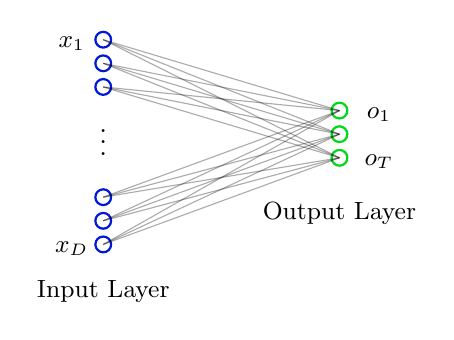
\begin{tikzpicture}
\foreach \x in {0.1,0.4,0.7} {
    \draw[dblue,thick,fill=white] (0,\x) circle (0.1cm);
}
\node at (0,1.5) {$\vdots$};
\node at (-0.4,0.05) {\small$x_D$};
\node at (-0.4,2.65) {\small$x_1$};
\node at (0, -0.5) {\small Input Layer};
\foreach \x in {2.1,2.4,2.7} {
    \draw[dblue,thick,fill=white] (0,\x) circle (0.1cm);
}
\foreach \x in {1.2,1.5,1.8} {
    \draw[dgreen,thick,fill=white] (3,\x) circle (0.1cm);
}
\node at (3.5,1.15) {\small$o_T$};
\node at (3.5,1.75) {\small$o_1$};
\node at (3, 0.5) {\small Output Layer};
\foreach \x in {1.2,1.5,1.8} {
    \foreach \y in {0.1,0.4,0.7} {
        \draw[black,opacity=0.33] (0,\y) -- (3,\x);
    }
}
\foreach \x in {1.2,1.5,1.8} {
    \foreach \y in {2.1,2.4,2.7} {
        \draw[black,opacity=0.33] (0,\y) -- (3,\x);
    }
}
\end{tikzpicture}
\end{center}

\end{frame}


\begin{frame}
\frametitle{Neural Networks}
\framesubtitle{Layers}

Layers are often given names based on what they do
\begin{itemize}
    \item Layer with above neurons ($a(v)=v$) called \emph{linear}
    \item Activation functions often considered own layer
\end{itemize}

\medskip

\begin{center}
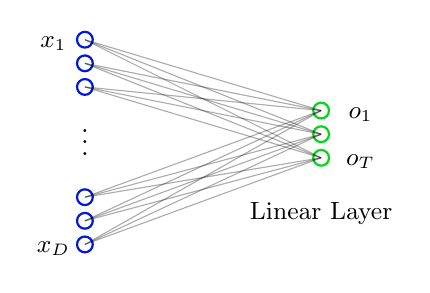
\begin{tikzpicture}
\foreach \x in {0.1,0.4,0.7} {
    \draw[dblue,thick,fill=white] (0,\x) circle (0.1cm);
}
\node at (0,1.5) {$\vdots$};
\node at (-0.4,0.05) {\small$x_D$};
\node at (-0.4,2.65) {\small$x_1$};
\foreach \x in {2.1,2.4,2.7} {
    \draw[dblue,thick,fill=white] (0,\x) circle (0.1cm);
}
\foreach \x in {1.2,1.5,1.8} {
    \draw[dgreen,thick,fill=white] (3,\x) circle (0.1cm);
}
\node at (3.5,1.15) {\small$o_T$};
\node at (3.5,1.75) {\small$o_1$};
\node at (3, 0.5) {\small Linear Layer};
\foreach \x in {1.2,1.5,1.8} {
    \foreach \y in {0.1,0.4,0.7} {
        \draw[black,opacity=0.33] (0,\y) -- (3,\x);
    }
}
\foreach \x in {1.2,1.5,1.8} {
    \foreach \y in {2.1,2.4,2.7} {
        \draw[black,opacity=0.33] (0,\y) -- (3,\x);
    }
}
\end{tikzpicture}
\end{center}

\end{frame}


\begin{frame}
\frametitle{Neural Networks}
\framesubtitle{Layers}

Can add \emph{hidden layers} to increase model capacity
\begin{itemize}
    \item Such networks are called \emph{multi-layer perceptrons} (\emph{MLPs})
    \item \emph{Deep neural networks} (\emph{DNNs}) have several such layers
\end{itemize}

\medskip

\begin{center}
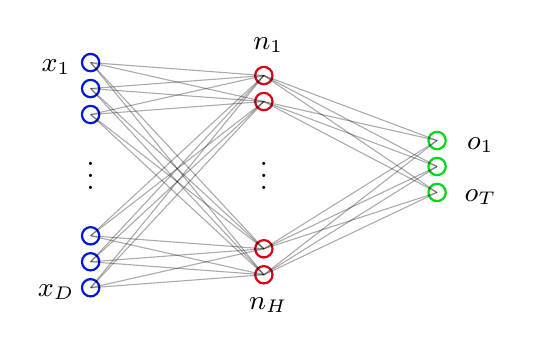
\begin{tikzpicture}[scale=1.1, every node/.style={scale=1.1}]
\foreach \x in {0.1,0.4,0.7} {
    \draw[dblue,thick,fill=white] (0,\x) circle (0.1cm);
}
\foreach \x in {0.25,0.55} {
    \draw[dred,thick,fill=white] (2,\x) circle (0.1cm);
}
\foreach \x in {2.25,2.55} {
    \draw[dred,thick,fill=white] (2,\x) circle (0.1cm);
}
\node at (0,1.5) {$\vdots$};
\node at (2,1.5) {$\vdots$};%
\node at (-0.4,0.05) {\small$x_D$};
\node at (-0.4,2.65) {\small$x_1$};
\node at (2.05,2.9) {\small$n_1$};
\node at (2.05,-0.1) {\small$n_H$};
\foreach \x in {2.1,2.4,2.7} {
    \draw[dblue,thick,fill=white] (0,\x) circle (0.1cm);
}
\foreach \x in {1.2,1.5,1.8} {
    \draw[dgreen,thick,fill=white] (4,\x) circle (0.1cm);
}
\node at (4.5,1.15) {\small$o_T$};
\node at (4.5,1.75) {\small$o_1$};
\foreach \x in {0.25,0.55} {
    \foreach \y in {0.1,0.4,0.7,2.1,2.4,2.7} {
        \draw[black,opacity=0.33] (0,\y) -- (2,\x);
    }
}
\foreach \x in {2.25,2.55} {
    \foreach \y in {0.1,0.4,0.7,2.1,2.4,2.7} {
        \draw[black,opacity=0.33] (0,\y) -- (2,\x);
    }
}
\foreach \x in {0.25,0.55} {
    \foreach \y in {1.2,1.5,1.8} {
        \draw[black,opacity=0.33] (2,\x) -- (4,\y);
    }
}
\foreach \x in {2.25,2.55} {
    \foreach \y in {1.2,1.5,1.8} {
        \draw[black,opacity=0.33] (2,\x) -- (4,\y);
    }
}
\end{tikzpicture}
\end{center}

\end{frame}


\begin{frame}
  \frametitle{Neural Networks}
  \framesubtitle{Layers}
  
  Assuming $D=1$ and $a(v)=$ ReLU
  \begin{itemize}
    \item Model is $T$ piecewise linear functions with $H$ kinks
    \item Same for $D>1$ but hard to visualize
  \end{itemize}

  \medskip

  \begin{center}
    \copyrightbox[b]
    {\includegraphics[width=10cm]{images/mlp-step}}
    {\centering Image from [3]}
\end{center}
  
  \end{frame}


\begin{frame}
\frametitle{Neural Networks}
\framesubtitle{Demo}

\begin{center}
    \copyrightbox[b]
    {\includegraphics[width=4.5cm]{images/mlp-classification}}
    {\centering Image from \href{http://cs.stanford.edu/people/karpathy/convnetjs/demo/classify2d.html}{cs.stanford.edu}} %
\end{center}

\end{frame}


\begin{frame}
  \frametitle{Neural Networks}
  \framesubtitle{Universal Approximators}
  
  MLPs are \emph{universal approximators} (depending on $H$ and $a(\cdot)$)
  \begin{itemize}
      \item Can represent any decision boundary (classification)
      \item Can approximate any function to any degree (regression)
  \end{itemize}
  
  \bigskip
  
  Does this solve our image classification problems?
  \begin{itemize}
      \item No because we have bad (low-level) feature vectors
      \item Garbage in, garbage out
  \end{itemize}
  
  \end{frame}


\begin{frame}
  \frametitle{Neural Networks}
  \framesubtitle{Universal Approximators}
  
  What if we use the raw images instead?
  \begin{itemize}
    \item Squeeze $32\times32\times3$ images to vectors $\vx$ with $\dim(\vx)=3072$
\end{itemize}

\bigskip
  
Also does not work
\begin{itemize}
    \item Shallow MLPs perform poorly
    \item Neither do deep MLPs (also poor scaling) %
\end{itemize}

\bigskip
MLP-based designs that work well exist though
\begin{itemize}
  \item More in a later lecture
\end{itemize}
  
  \end{frame}


\begin{frame}
\frametitle{Neural Networks}
\framesubtitle{Computational Graphs}

The term \enquote{neural network} is misleading
\begin{itemize}
    \item Biological neurons are much more complex [1]
    \item Modern (deep) neural networks have evolved a lot
\end{itemize}

\bigskip

Better to think of modern neural networks as
\begin{itemize}
    \item Compositions of scalar sub-functions (\emph{units})
    \item That form a directed acyclic computational graph
    \item And grouped into layers depending on distance from input
\end{itemize}

\end{frame}


\begin{frame}
\frametitle{Neural Networks}
\framesubtitle{Computational Graphs -- Example}


\[
    o=f(x)=f(g_1(h_1(x), h_2(x)), g_2(h_2(x), h_3(x)))
\]

\bigskip

\begin{center}
    \copyrightbox[b]
    {\includegraphics[width=4.5cm]{images/nn-graph}}
    {\centering Image from wikipedia}
\end{center}

\end{frame}


\begin{frame}
\frametitle{Neural Networks}
\framesubtitle{Computational Graphs}

Granularity can be chosen freely %
\begin{itemize}
    \item We might define $g(\vx)=\vw\cdot\vx+b$
    \item Or $g(\vx)=h_1(x_1)+\cdots+h_D(x_D)+b$ with $h_d(x_d)=w_d x_d$
    \item Or whatever we want really %
\end{itemize}

\bigskip

We will vary granularity depending on context
\begin{itemize}
    \item More granularity helps understanding training process
    \item Implementations are less granular (parallel computations)
\end{itemize}

\end{frame}


{
\setbeamertemplate{footline}{}
\begin{frame}

\begin{tikzpicture}[remember picture,overlay]
\fill[white] (current page.north west) rectangle (current page.south east);
\end{tikzpicture}

\begin{center}
\textcolor[rgb]{0.9,0.9,0.9}{blank page}
\end{center}

\end{frame}
}


\begin{frame}
\frametitle{Gradient Computation}

Training involves computing $\nabla L(\bth)$ in every iteration
\begin{itemize}
  \item Many iterations required to train networks
  \item Computation must be exact and efficient
\end{itemize}

\end{frame}


\begin{frame}
\frametitle{Gradient Computation}
\framesubtitle{Parameter Initialization}

Got to initialize all parameters first
\begin{itemize}
  \item Multiplicative \emph{weights} $\vw_1\cdots\vw_H$ and $\vw_1\cdots\vw_T$ %
  \item Additive \emph{biases} $b_1\cdots b_H$ and $b_1\cdots b_T$ %
\end{itemize}

\bigskip

Want to preserve signal strength throughout network
\begin{itemize}
  \item Avoid numerical issues (floating point math)
  \item Prevent \emph{exploding} or \emph{vanishing gradients}
\end{itemize}
  
\bigskip

Biases are not critical
\begin{itemize}
  \item Simply set to $0$ initially
\end{itemize}
  
  \end{frame}


\begin{frame}
\frametitle{Gradient Computation}
\framesubtitle{Parameter Initialization}

Weights are critical (multiplicative effect on output)
\begin{itemize}
  \item Signal will vanish/explode if weights too small/large
  \item The deeper the network, the bigger the problem
\end{itemize}

\medskip

\begin{center}
  \copyrightbox[b]
  {\includegraphics[width=8cm]{images/signal-strength}} %
  {\centering Image from [3].}
\end{center}
  
\end{frame}


\begin{frame}
  \frametitle{Gradient Computation}
  \framesubtitle{Parameter Initialization}
  
    Sample weights from $\mathcal{N}(0,\sigma)$ to avoid issues
    \begin{itemize}
        \item Optimal $\sigma$ depends on number of connections and $a(\cdot)$ %
        \item See [3] for details if interested
    \end{itemize}
  
    \bigskip
    Note that this preserves signal only initially
    \begin{itemize}
      \item Weights change during training
      \item Why normalization layers are important (more later)
    \end{itemize}
    
  \end{frame}


\begin{frame}
\frametitle{Gradient Computation}
\framesubtitle{Numerical Gradients}

One way to obtain $\nabla L(\bth)$ is \emph{numerical differentiation}
\begin{itemize}
    \item $\nabla L_p(\bth)=(L(\bth+\boldsymbol{1}_p\epsilon)-L(\bth))/\epsilon$ for $p\in[1,\dim(\bth)]$ %
    \item Vector $\boldsymbol{1}_p$ is $1$ at position $p$ and $0$ otherwise
    \item Follows directly from definition of the derivative %
\end{itemize}

\bigskip

Practical considerations
\begin{itemize}
    \item $\epsilon$ should be close to $0$ while avoiding numerical issues %
    \item $\nabla L_p(\bth)=(L(\bth+\boldsymbol{1}_p\epsilon)-L(\bth-\boldsymbol{1}_p\epsilon))/2\epsilon$ preferable %
\end{itemize}

\end{frame}


\begin{frame}
\frametitle{Gradient Computation}
\framesubtitle{Numerical Gradients}

Trivial to implement

\bigskip

Only an approximation ($\epsilon$ cannot be arbitrarily small)

\bigskip

Too inefficient in practice
\begin{itemize}
    \item Must evaluate $L$ $\dim(\bth)+1$ times
    \item Complex networks have millions of parameters
\end{itemize}

\end{frame}


\begin{frame}
\frametitle{Gradient Computation}
\framesubtitle{Analytic Gradients}

We thus would prefer the \emph{analytic gradient}
\begin{itemize}
    \item Obtain $\nabla L$ analytically using calculus %
\end{itemize}

\bigskip

Can compute $\nabla L(\bth)$ directly
\begin{itemize}
    \item Accurate (no approximation) %
    \item Potentially much more efficient (single evaluation) %
\end{itemize}

\end{frame}


\begin{frame}
\frametitle{Gradient Computation}
\framesubtitle{Derivatives in Graphs}

Neural networks are computational graphs
\begin{itemize}
    \item As are loss function defined for them
\end{itemize}

\bigskip

Derivatives in such graphs can be computed iteratively
\begin{itemize}
    \item Recursive application of the chain rule
    \item Recall that if $F(x)=f(g(x))$ then $F'(x)=f'(g(x))g'(x)$
\end{itemize}

\bigskip

To compute gradients in such graphs we
\begin{itemize}
    \item Evaluate the graph and store local results (\emph{forward pass})
    \item Aggregate local gradients (\emph{backward pass})
\end{itemize}

\end{frame}


\begin{frame}
\frametitle{Gradient Computation}
\framesubtitle{Derivatives in Graphs}

Simple example with $e(a,\,b)=(a+b)(b+1)$

\medskip

\begin{center}
    \copyrightbox[b]
    {\includegraphics[width=7cm]{images/backprop-tree-def}}
    {\centering Image from \href{https://colah.github.io/posts/2015-08-Backprop/}{colah.github.org}}
\end{center}

\end{frame}


\begin{frame}
\frametitle{Gradient Computation}
\framesubtitle{Derivatives in Graphs}

Forward pass with $a=2$ and $b=1$

\medskip


\begin{center}
    \copyrightbox[b]
    {\includegraphics[width=7cm]{images/backprop-tree-eval}}
    {\centering Image from \href{https://colah.github.io/posts/2015-08-Backprop/}{colah.github.org}}
\end{center}

\end{frame}


\begin{frame}
\frametitle{Gradient Computation}
\framesubtitle{Derivatives in Graphs}

Every node can compute \emph{local gradients} independently
\begin{itemize}
    \item $\partial f/\partial x$ means partial derivative $f_x$ %
\end{itemize}


\medskip

\begin{center}
    \copyrightbox[b]
    {\includegraphics[width=7.5cm]{images/backprop-tree-eval-derivs}}
    {\centering Image from \href{https://colah.github.io/posts/2015-08-Backprop/}{colah.github.org}}
\end{center}

\end{frame}


\begin{frame}
\frametitle{Gradient Computation}
\framesubtitle{Derivatives in Graphs}

To obtain $\nabla e(2,1)$ we use the multivariate chain rule

\bigskip

We calculate $\nabla e_a(2,1)$ by
\begin{itemize}
    \item Multiplying local gradients along every path from $a$ to $e$
    \item Summing over all resulting values
\end{itemize}

\bigskip

Same for $e_b$ (and all other variables in general) %

\end{frame}


\begin{frame}
\frametitle{Gradient Computation}
\framesubtitle{Derivatives in Graphs}

$e_a(2,1)=c_a(2,1)\cdot e_c(2,1)=1\cdot 2=2$


\medskip

\begin{center}
    \copyrightbox[b]
    {\includegraphics[width=7.5cm]{images/backprop-tree-eval-derivs}}
    {\centering Image from \href{https://colah.github.io/posts/2015-08-Backprop/}{colah.github.org}}
\end{center}

\end{frame}


\begin{frame}
\frametitle{Gradient Computation}
\framesubtitle{Derivatives in Graphs}

$e_b(2,1)=c_b(2,1)\cdot e_c(2,1)+ d_b(2,1)\cdot e_d(2,1)=2+3=5$

\medskip

\begin{center}
    \copyrightbox[b]
    {\includegraphics[width=7.5cm]{images/backprop-tree-eval-derivs}}
    {\centering Image from \href{https://colah.github.io/posts/2015-08-Backprop/}{colah.github.org}}
\end{center}

\end{frame}


\begin{frame}
\frametitle{Gradient Computation}
\framesubtitle{Derivatives in Graphs}

Can use the same algorithm to compute $L(\bth)$

\bigskip

Recall that the loss is an average over $S$ samples
\begin{itemize}
    \item $L(\bth)=1/S\cdot\sum_s H(\vo^s,\text{softmax}(f(\vx^s;\bth)))$
\end{itemize}

\bigskip

So $\nabla L(\bth)$ is average of individual $\nabla H(\bth)$
\begin{itemize}
    \item Compute $\nabla H(\bth)$ for all $s$ and average
    \item Of course this applies to loss functions in general
\end{itemize}

\end{frame}


\begin{frame}
\frametitle{Gradient Computation}
\framesubtitle{Derivatives in Graphs}

To calculate $\nabla H(\bth)$ we
\begin{itemize}
    \item Decompose the NN to simple functions
    \item Do the same for the softmax and cross-entropy
    \item Stack both to obtain a combined graph
    \item Use the same algorithm as above
\end{itemize}

\end{frame}


\begin{frame}
\frametitle{Gradient Computation}
\framesubtitle{Derivatives in Graphs}

Neural networks are graphs of simple functions
\begin{itemize}
    \item Can decompose the inner products %
\end{itemize}

\bigskip

\begin{center}
\begin{tabular}{ll} \toprule
$f$ & $f'$ \\ \midrule
$x_1+x_2$ & $1$ \\
$x_1x_2$ & $x_2$ and $x_1$ \\ %
$\max(0,x)$ & $0$ or $1$ \\ \bottomrule %
\end{tabular}
\end{center}

\end{frame}


\begin{frame}
\frametitle{Gradient Computation}
\framesubtitle{Derivatives in Graphs}

As are the cross-entropy and softmax functions

\bigskip

\begin{center}
\begin{tabular}{ll} \toprule
$f$ & $f'$ \\ \midrule
$\exp(x)$ & $\exp(x)$ \\
$\ln(x)$ & $1/x$ \\
$x_1/x_2$ & $1/x_2$ and $-x_1/x_2^2$ \\ \bottomrule
\end{tabular}
\end{center}

\end{frame}


\begin{frame}
\frametitle{Gradient Computation}
\framesubtitle{Derivatives in Graphs}

Linear classifier with $D=2$ and $T=2$ %


\bigskip

\begin{center}
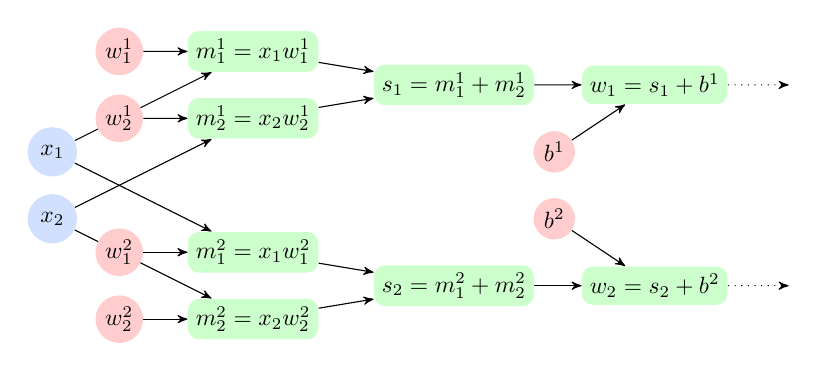
\begin{tikzpicture}[->,>=stealth',scale=0.85, every node/.style={scale=0.85}]
\tikzset{inpt/.style={circle,fill=xblue,draw=none}}
\tikzset{param/.style={circle,fill=xred,draw=none}}
\tikzset{comp/.style={fill=xgreen,draw=none,rounded corners}}
\def \h {1.5}
\def \w {1.5}
\node[inpt] at (0,1.5) (in1) {$x_1$};
\node[inpt] at (0,0.5) (in2) {$x_2$};
\node[param,inner sep=1.5pt] at (1,3) (w11) {$w^1_1$};
\node[param,inner sep=1.5pt] at (1,2) (w12) {$w^1_2$};
\node[comp] at (3,3) (dpm11) {$m^1_1=x_1w^1_1$};
\node[comp] at (3,2) (dpm12) {$m^1_2=x_2w^1_2$};
\begin{scope}[on background layer]
\draw (in1) -- (dpm11);
\draw (w11) -- (dpm11);
\draw (in2) -- (dpm12);
\draw (w12) -- (dpm12);
\end{scope}
\node[comp] at (6,2.5) (dps1) {$s_1=m^1_1+m^1_2$};
\draw (dpm11) -- (dps1);
\draw (dpm12) -- (dps1);
\node[param,inner sep=2pt] at (7.5,1.5) (b1) {$b^1$};
\node[comp] at (9,2.5) (bias1) {$w_1=s_1+b^1$};
\draw (dps1) -- (bias1);
\draw (b1) -- (bias1);
\draw[dotted] (bias1) -- (11,2.5);
\node[param,inner sep=1.5pt] at (1,0) (w21) {$w^2_1$};
\node[param,inner sep=1.5pt] at (1,-1) (w22) {$w^2_2$};
\node[comp] at (3,0) (dpm21) {$m^2_1=x_1w^2_1$};
\node[comp] at (3,-1) (dpm22) {$m^2_2=x_2w^2_2$};
\begin{scope}[on background layer]
\draw (in1) -- (dpm21);
\draw (w21) -- (dpm21);
\draw (in2) -- (dpm22);
\draw (w22) -- (dpm22);
\end{scope}
\node[comp] at (6,-0.5) (dps2) {$s_2=m^2_1+m^2_2$};
\draw (dpm21) -- (dps2);
\draw (dpm22) -- (dps2);
\node[param,inner sep=2pt] at (7.5,0.5) (b2) {$b^2$};
\node[comp] at (9,-0.5) (bias2) {$w_2=s_2+b^2$};
\draw (dps2) -- (bias2);
\draw (b2) -- (bias2);
\draw[dotted] (bias2) -- (11,-0.5);
\end{tikzpicture}
\end{center}

\end{frame}


\begin{frame}
\frametitle{Gradient Computation}
\framesubtitle{Derivatives in Graphs}

\enquote{Attached} softmax and cross-entropy

\bigskip

\begin{center}
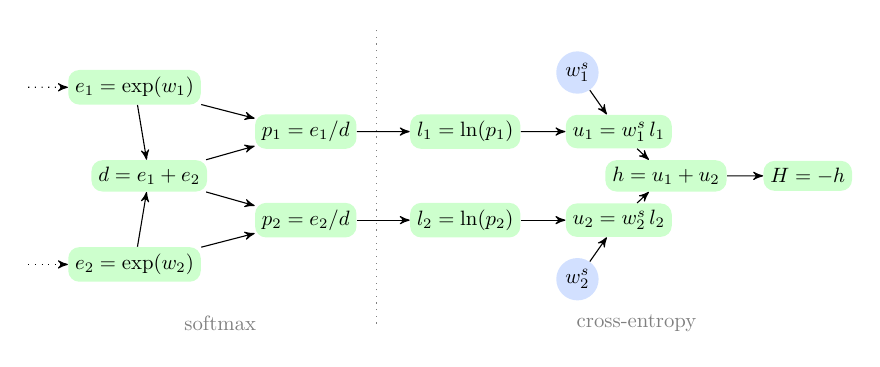
\begin{tikzpicture}[->,>=stealth',scale=0.75, every node/.style={scale=0.75}]
\tikzset{inpt/.style={circle,fill=xblue,draw=none}}
\tikzset{param/.style={circle,fill=xred,draw=none}}
\tikzset{comp/.style={fill=xgreen,draw=none,rounded corners}}
\node[comp] at (0,3) (exp1) {$e_1=\exp(w_1)$};
\draw[dotted] (-1.8,3) -- (exp1);
\node[comp] at (0,0) (exp2) {$e_2=\exp(w_2)$};
\draw[dotted] (-1.8,0) -- (exp2);
\node[comp] at (0.25,1.5) (sum1) {$d=e_1+e_2$};
\draw (exp1) -- (sum1);
\draw (exp2) -- (sum1);
\node[comp] at (2.9,2.25) (p1) {$p_1=e_1/d$};
\node[comp] at (2.9,0.75) (p2) {$p_2=e_2/d$};
\draw (exp1) -- (p1);
\draw (sum1) -- (p1);
\draw (exp2) -- (p2);
\draw (sum1) -- (p2);
\node[text=gray] at (1.45,-1) {softmax};
\draw[dotted,gray,-] (4.1,-1) -- (4.1,4);
\node[comp] at (5.6,2.25) (l1) {$l_1=\ln(p_1)$};
\node[comp] at (5.6,0.75) (l2) {$l_2=\ln(p_2)$};
\draw (p1) -- (l1);
\draw (p2) -- (l2);
\node[inpt,inner sep=2pt] at (7.5,3.25) (wt1) {$w^s_1$};
\node[comp] at (8.2,2.25) (m1) {$u_1=w^s_1\,l_1$};
\draw (wt1) -- (m1);
\draw (l1) -- (m1);
\node[inpt,inner sep=2pt] at (7.5,-0.25) (wt2) {$w^s_2$};
\node[comp] at (8.2,0.75) (m2) {$u_2=w^s_2\,l_2$};
\draw (wt2) -- (m2);
\draw (l2) -- (m2);
\node[comp] at (9,1.5) (sum2) {$h=u_1+u_2$};
\draw (m1) -- (sum2);
\draw (m2) -- (sum2);
\node[comp] at (11.4,1.5) (ce) {$H=-h$};
\draw (sum2) -- (ce);
\node[text=gray] at (8.5,-1) {cross-entropy};
\end{tikzpicture}
\end{center}

\end{frame}


\begin{frame}
\frametitle{Gradient Computation}
\framesubtitle{Derivatives in Graphs}

Graph is dense
\begin{itemize}
    \item Must sum over several paths per partial derivative
    \item Number of paths grows exponentially with graph complexity
    \item Above algorithm not efficient enough for large networks
\end{itemize}

\end{frame}


\begin{frame}
\frametitle{Gradient Computation}
\framesubtitle{Derivatives in Graphs}

\emph{Reverse-mode differentiation} solves this problem
\begin{itemize}
    \item Computes derivatives of output node wrt.~all other nodes
    \item Efficiently by touching every edge only once
    \item Called \emph{backpropagation} in neural network community
\end{itemize}

\bigskip

Achieved by
\begin{itemize}
    \item Starting at the output (loss) node
    \item Propagating local gradients backwards to input nodes
    \item Storing intermediate results for efficiency
\end{itemize}


\end{frame}


\begin{frame}
\frametitle{Gradient Computation}
\framesubtitle{Derivatives in Graphs}

Start at output node $e$ and move towards inputs

\bigskip

At every node $n$
\begin{itemize}
    \item For every child $c$, compute local gradient $l_c=\partial n/\partial c$ %
    \item For every child $c$, compute $m_c=l_c\cdot\partial e/\partial n$ ($\partial e/\partial e=1$)
    \item Compute $\partial e/\partial c$ as sum over all $m_c$
\end{itemize}

\end{frame}


\begin{frame}
\frametitle{Gradient Computation}
\framesubtitle{Derivatives in Graphs}


\begin{center}
    \copyrightbox[b]
    {\includegraphics[width=8cm]{images/backprop-tree-backprop}}
    {\centering Image from \href{https://colah.github.io/posts/2015-08-Backprop/}{colah.github.org}}
\end{center}

\end{frame}


\begin{frame}
\frametitle{Gradient Computation}
\framesubtitle{Derivatives in Graphs}

Resulting patterns in gradient flow
\begin{itemize}
    \item \texttt{Add} distributes gradients unchanged to all inputs %
    \item \texttt{Max} routes gradient unchanged to largest input %
    \item \texttt{Multiply} multiplies with switched inputs
\end{itemize}

\medskip

\begin{center}
    \copyrightbox[b]
    {\includegraphics[width=5cm]{images/gradient-flow}}
    {\centering Image from cs231n.github.io}
\end{center}

\end{frame}


\begin{frame}
\frametitle{Gradient Computation}
\framesubtitle{Derivatives in Graphs}

Neural networks are always trained using backpropagation
\begin{itemize}
    \item Can increase efficiency by many magnitudes %
    \item Makes training huge (deep) neural networks feasible
\end{itemize}

\bigskip

In practice
\begin{itemize}
    \item Graph composition not as fine (vectorization) %
    \item $\nabla H(\bth)$ computed in parallel for all $s$ (data parallelism)
\end{itemize}

\end{frame}


\renewcommand\emph[1]{\oldemph{#1}}

\begin{frame}
\frametitle{Bibliography}

[1] Brunel et al. Single neuron dynamics and computation. 2014.

\smallskip

[2] Prince. Computer Vision Models. 2012.

\smallskip

[3] Prince. Understanding Deep Learning. 2023.

\end{frame}


\end{document}
